\documentclass[conference,a4paper]{IEEEtran}
\IEEEoverridecommandlockouts
% Double-Blind Review Compliance: Author information is anonymized in accordance with conference guidelines.

\usepackage{cite}
\usepackage{amsmath,amssymb,amsfonts}
\usepackage{algorithmic}
\usepackage{graphicx}
\usepackage{textcomp}
\usepackage{xcolor}
\usepackage{booktabs}
\usepackage{multirow}
\usepackage{url}
\usepackage{microtype}

\def\BibTeX{{\rm B\kern-.05em{\sc i\kern-.025em b}\kern-.08em
    T\kern-.1667em\lower.7ex\hbox{E}\kern-.125emX}}

\begin{document}

\title{Multiscale Computer Vision Ecosystem for Generalized Coconut Pathology Detection: A Context-Aware Architecture for Precision Agriculture}

\author{
\IEEEauthorblockN{Anonymous Authors}
\IEEEauthorblockA{\textit{Department of Software Engineering} \\
\textit{Faculty of Computing, Sri Lanka Institute of Information Technology}\\
Malabe, Sri Lanka \\
Email: anonymized@my.sliit.lk}
}

\maketitle

\begin{abstract}
The coconut palm (\textit{Cocos nucifera} L.) is an essential pillar of tropical agricultural economies, dietary security, and export revenue. However, crop yields face severe threats from aggressive biological pathogens, notably Weligama Coconut Leaf Wilt Disease (WCLWD), Bud Rot, Stem Bleeding, and Leaf Rot. Existing monitoring approaches suffer from a scale bifurcation gap: high-altitude aerial surveillance via Unmanned Aerial Vehicles (UAVs) provides macroscopic coverage but lacks lesion-level diagnostic resolution, whereas mobile deep learning classifiers operate in isolation and depend on erratic network connectivity. This paper presents an end-to-end, multiscale computer vision ecosystem bridging macroscopic aerial surveillance with offline-first microscopic edge intelligence. At the macroscopic tier (System~A), deterministic mathematical morphology, integrating Canonical Excess-Green (ExG) chromatic canopy isolation, Euclidean Distance Transform (EDT) topological crown extraction, and a Moving-Window Local Spatial Z-Score Anomaly Engine, enables a zero-annotation physical tree census and early stress hotspot localization without deep neural network overhead. At the microscopic tier (System~B), an asymmetric Full-Integer INT8 Post-Training Quantized MobileNetV2 architecture (2.71~MB) combined with Temperature-Scaled Shannon Entropy Out-of-Distribution (OOD) gating delivers rapid foliar diagnostics on budget mobile processors while rejecting non-foliar visual noise. Diagnostic telemetry is orchestrated through a closed-loop biosecurity bridge combining local SQLite offline queuing with asynchronous Firebase synchronization and Coconut Research Institute (CRI) treatment protocols. Empirical validations across commercial plantations (Ambakele Research Station) demonstrate rapid crown extraction (938 discrete palms isolated in 105.2ms), localized stress hotspot detection within a 35m spatial radius (21 early stress hotspots at $Z < -2.0$), and a 99.58\% Top-1 diagnostic accuracy across pathological classes ($\kappa = 0.9947$), delivering an affordable and robust biosecurity architecture for smallholder precision agriculture.
\end{abstract}

\begin{IEEEkeywords}
Precision Agriculture, Coconut Pathology, Multiscale Computer Vision, Euclidean Distance Transform, Vegetation Indices, Edge AI, Out-of-Distribution Detection.
\end{IEEEkeywords}

\section{Introduction}
The coconut palm (\textit{Cocos nucifera} L.) is a major agricultural commodity and export product in tropical developing nations. In Sri Lanka, coconut cultivation covers approximately 402,649 hectares (representing 21\% of total agricultural land), primarily clustered in the traditional ``Coconut Triangle'' (Kurunegala, Puttalam, Gampaha) and the southern ``Mini Coconut Triangle'' (Matara, Beliatta, Ranna) \cite{b1}. Despite its economic value, the industry faces severe stability challenges driven by extreme weather variability, estate land fragmentation, and aggressive biological pathogens.

Among these threats, Weligama Coconut Leaf Wilt Disease (WCLWD), a phytoplasma-mediated systemic disorder closely related to sugarcane grassy shoot phytoplasma, has caused widespread yield losses in southern Sri Lanka \cite{b5}. Because early phytoplasma symptoms involve subtle leaflet flaccidity and uneven chlorosis, they frequently mimic benign magnesium and nitrogen deficiencies, misleading visual inspections \cite{b11,b18}. Concurrently, lethal fungal and oomycete infections such as Bud Rot (\textit{Phytophthora palmivora}), Stem Bleeding (\textit{Ceratocystis paradoxa}), and Leaf Rot (\textit{Colletotrichum gloeosporioides}) damage internal vascular tissues and apical meristems before outer canopy collapse is visible. In severe outbreaks, phytosanitary authorities such as the Coconut Research Institute (CRI) mandate the felling of infected palms to contain transmission \cite{b6}.

Current agronomic monitoring protocols face two primary structural bottlenecks, termed here as the \textbf{Scale Bifurcation Gap}:
\begin{enumerate}[\IEEEsetlabelwidth{1)}]
    \item \textit{Macroscopic Disconnect:} High-altitude Unmanned Aerial Vehicles (UAVs) and satellite multispectral sensors can survey 50--100 hectare estates rapidly \cite{b10,b13}. However, deploying standard deep learning object detectors (e.g., YOLOv11, Mask R-CNN) on 20-megapixel drone orthomosaics requires extensive manual bounding-box annotations, induces memory exhaustion on serverless cloud functions, and cannot verify microscopic pathogen etiologies beneath the crown.
    \item \textit{Microscopic Isolation:} Ground-level mobile deep learning models enable lesion-level diagnosis \cite{b3,b9}. However, they function in spatial isolation, rely on uncoordinated manual patrols, and fail in rural zero-connectivity zones. Furthermore, standard softmax activations exhibit uncalibrated overconfidence when presented with uncontrolled field noise (mud, human fingers, sun glare) \cite{b12}.
\end{enumerate}

To resolve these challenges, this paper presents a multiscale computer vision ecosystem that unifies macroscopic aerial surveillance with offline-first microscopic edge diagnostics. The core contributions are:
\begin{itemize}
    \item \textbf{Deterministic Macroscopic Topology (System A):} A lightweight mathematical morphology pipeline combining Canonical Excess-Green (ExG) chromatic filtering and Euclidean Distance Transform (EDT) peak extraction that achieves an automated physical tree census on standard planting grids without requiring annotated neural network training data.
    \item \textbf{Local Spatial Z-Score Anomaly Engine:} A moving-window spatial statistical filter that isolates early canopy stress clusters against local neighborhood baseline vigor, mitigating background soil reflectance bias.
    \item \textbf{Quantized Edge Diagnostics with OOD Gating (System B):} An asymmetric Full-Integer INT8 Post-Training Quantized MobileNetV2 model (disk footprint compressed by 75.0\% to 2.71~MB) integrated with Temperature-Scaled Shannon Entropy gating to filter non-foliar visual artifacts as ``Ambiguous Foliage''.
    \item \textbf{Closed-Loop Biosecurity Bridge:} An asynchronous orchestration protocol linking macroscopic UAV hotspot coordinates to mobile field-scout GPS dispatches, supported by an offline-first SQLite synchronization engine and CRI agronomic remediation protocols.
\end{itemize}

% =========================================================================
\section{Related Work \& Phytopathological Context}

\subsection{Deep Learning in Foliar Pathology}
Recent studies in precision agriculture highlight the efficacy of deep convolutional networks for foliar disease classification. Daga et al. \cite{b1} proposed DeepSeqCoco, an optimized mobile architecture using hybrid SGD-Adam optimization that reduced inference latency on edge devices. Alkhawaji et al. \cite{b9} and Singh et al. \cite{b10} evaluated deep convolutional backbones for palm disease classification, reporting high validation accuracies on curated benchmarks. Similarly, the hybrid NNSVCLD framework \cite{b3} combined deep feature extraction with Support Vector Machines (SVM) to classify bud rot and leaf blight with 99.4\% accuracy.

However, existing frameworks encounter practical deployment challenges. Computationally heavy architectures (e.g., EfficientNet-B7 or Inception-ResNet-V2 \cite{b12}) cause thermal throttling and battery drain on budget smartphone processors. Furthermore, standard mobile classifiers lack out-of-distribution (OOD) rejection mechanisms, producing high-confidence false predictions on non-foliar visual artifacts.

\subsection{Aerial Remote Sensing in Plantation Agriculture}
At the macroscopic canopy scale, UAV multispectral imaging combined with Object-Based Image Analysis (OBIA) has shown substantial efficacy in detecting canopy-level stress \cite{b13}. Divyanth et al. \cite{b13} demonstrated that Near-Infrared (NIR) vegetation indices isolate internal cellular mesophyll collapse in WCLWD-affected palms prior to visual chlorosis. Advanced segmentation techniques such as JASS-Net \cite{b14} and TKRnet \cite{b15} have achieved strong canopy delineation. However, executing sliding-window neural inference over high-resolution drone orthomosaics requires dedicated GPU cloud infrastructure, making continuous deployment economically prohibitive for smallholder cooperatives.

\subsection{Etiological Modeling: A Multiscale Disease Complex}
Crucially, phytopathological management in Sri Lanka requires modeling diseases across spatial scales. WCLWD manifests macroscopically through canopy thinning, flaccidity of the lower frond whorls, and generalized chlorosis. However, secondary foliar necrosis and opportunistic fungal blights (specifically \textit{Colletotrichum} Leaf Rot and \textit{Pestalotiopsis} Gray Leaf Spot) rapidly colonize immunocompromised palms. Consequently, a robust biosecurity framework must detect canopy vigor decline aerially and subsequently verify the specific active necrotic agent on the ground across a verified 6-class pathological taxonomy: (1) Bud Rot, (2) Stem Bleeding, (3) Leaf Rot, (4) Bud Root Dropping, (5) Gray Leaf Spot, and (6) Healthy Baseline.

% =========================================================================
\section{System A: Macroscopic Aerial Surveillance}

System~A functions as the macroscopic intelligence layer, ingesting 4K RGB and multispectral orthomosaics covering expansive 50--100 hectare plantation blocks. The overall architecture is depicted in Fig.~\ref{fig:architecture}.

\begin{figure*}[t]
\centering
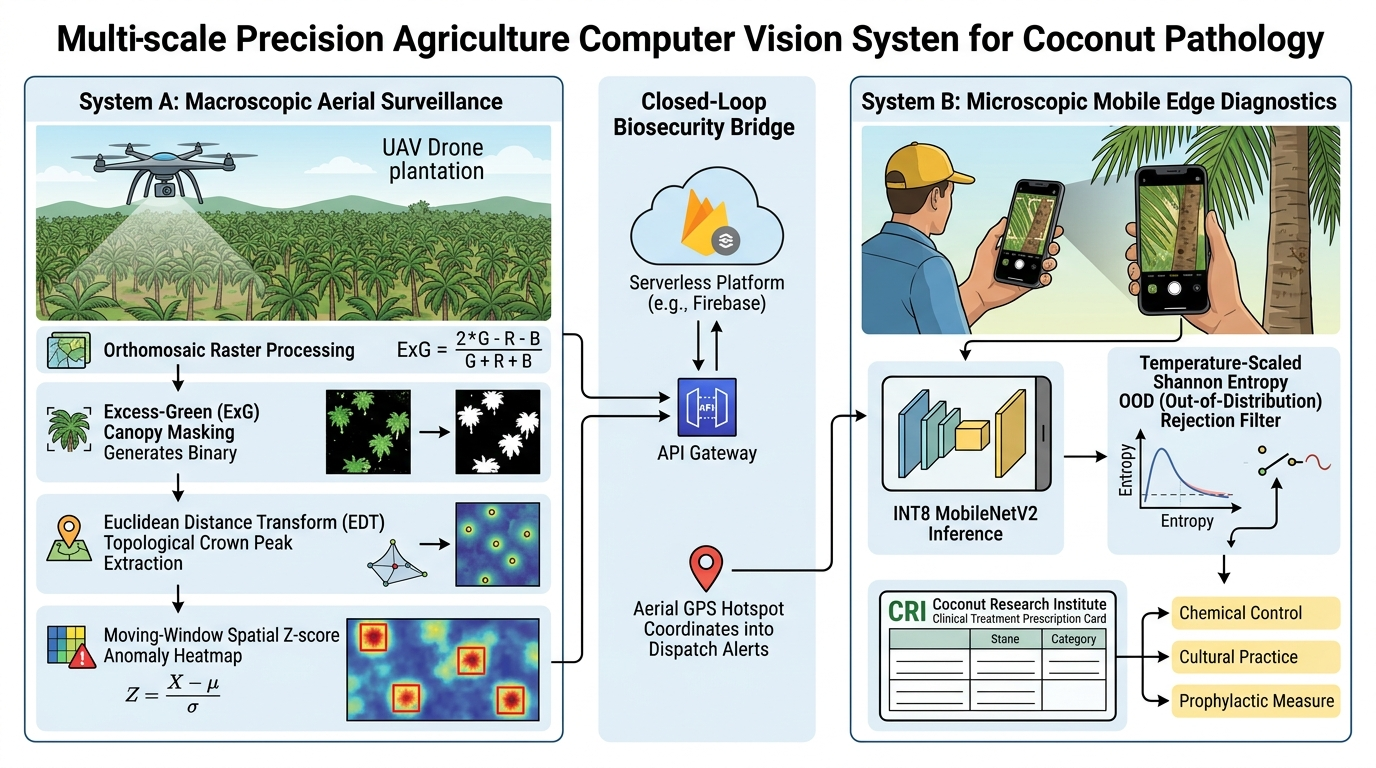
\includegraphics[width=0.88\textwidth]{fig1.png}
\caption{End-to-End Multiscale Architecture: Macroscopic UAV spectral segmentation and deterministic EDT crown extraction (System A) dispatch georeferenced anomaly hotspots to mobile field scouts for INT8 microscopic classification and CRI advisory delivery (System B).}
\label{fig:architecture}
\end{figure*}

\subsection{Strategy A: Radiometric Canopy Isolation}
Commercial coconut plantations in Sri Lanka adhere to an $8.0\text{m} \times 8.0\text{m}$ grid, causing 60\% to 70\% of raw aerial imagery to consist of non-canopy background (sandy loam soil, gravel roads, drying yards, and shadows). Unfiltered global index calculations severely depress mean spectral values due to soil reflectance.

To eliminate background contamination, raw RGB channels ($R, G, B \in [0, 255]$) are normalized into chromatic coordinates:
\begin{equation}
r = \frac{R}{\Sigma_{\text{rgb}}}, \quad g = \frac{G}{\Sigma_{\text{rgb}}}, \quad b = \frac{B}{\Sigma_{\text{rgb}}}
\label{eq:chromatic}
\end{equation}
where $\Sigma_{\text{rgb}} = R+G+B$. The Normalized Excess-Green Index ($\text{ExG}$) is derived to amplify photosynthetic tissue dominance:
\begin{equation}
\text{ExG} = 2g - r - b
\label{eq:exg}
\end{equation}
A binary Canonical Physical Canopy Mask $\mathcal{M}(x,y) \in \{0, 1\}$ is generated via empirical gating and Otsu global binarization:
\begin{equation}
\mathcal{M}(x,y) = 
\begin{cases}
1, & \text{if } \text{ExG}(x,y) \ge \tau_{\text{otsu}} \;\wedge\; g(x,y) > r(x,y) \\
0, & \text{otherwise}
\end{cases}
\label{eq:canopy_mask}
\end{equation}
All non-canopy pixels ($\mathcal{M}=0$) are mapped to a neutral zero-reflectance dark slate tensor, resolving soil reflectance bias while reducing downstream processing memory.

\subsection{Strategy B: Deterministic Morphological Crown Extraction}
Rather than training computationally intensive convolutional object detectors, System~A exploits a fundamental geometric invariant of the monocot palm: its radial canopy symmetry. For all confirmed canopy pixels in $\mathcal{M}$, the Euclidean Distance Transform (EDT) computes the shortest distance to the nearest background boundary:
\begin{equation}
D(p) = \min_{q \notin \mathcal{M}} \|p - q\|_2, \quad \forall p \in \mathcal{M}
\label{eq:edt}
\end{equation}
Because fronds radiate outward from the apical meristem, $D(p)$ generates a topological cone whose local maximum coincides with the crown center. To eliminate high-frequency leaflet noise while preserving crown-level peaks, Gaussian topological smoothing is applied:
\begin{equation}
D_{\text{smooth}} = D * G_\sigma, \quad G_\sigma = \frac{1}{2\pi\sigma^2} \exp\left(-\frac{x^2+y^2}{2\sigma^2}\right)
\label{eq:gaussian}
\end{equation}
with $\sigma = 2.2$. Individual palm apices $\mathcal{P}$ are extracted using a Spatial Local Maxima Peak filter over an agronomic footprint $\mathcal{F}$ of size $(2d_{\min} + 1) \times (2d_{\min} + 1)$:
\begin{equation}
\begin{split}
\mathcal{P} = \Big\{ p \in \mathcal{M} \;\Big|\; & D_{\text{smooth}}(p) = \max_{q \in \mathcal{F}(p)} D_{\text{smooth}}(q) \\
& \wedge\; D_{\text{smooth}}(p) \ge \delta_{\text{depth}} \Big\}
\end{split}
\label{eq:peaks}
\end{equation}
where $d_{\min} \approx 26\text{ pixels}$ matches the physical 8.0m spacing at standard orthomosaic scale, and $\delta_{\text{depth}} = 6.0\text{ pixels}$ excludes isolated weeds. This deterministic process produces an immutable geospatial coordinate $(\text{lat}_i, \text{lng}_i)$ and crown radius $r_i$ for every physical tree without manual annotations.

\subsection{Spectral Index Formulations}
For consumer RGB drones, the Visible Atmospherically Resistant Index (VARI) estimates vegetative vigor while compensating for coastal atmospheric aerosol scattering:
\begin{equation}
\text{VARI} = \frac{G - R}{G + R - B}
\label{eq:vari}
\end{equation}
For multispectral sensors, linear sensor-space Normalized Difference Vegetation Index (NDVI) is computed to detect cellular mesophyll decay:
\begin{equation}
\text{NDVI} = \frac{\text{NIR} - R}{\text{NIR} + R}
\label{eq:ndvi}
\end{equation}

\subsection{Strategy C: Moving-Window Local Spatial Z-Score Engine}
Pathological infection spreads in localized spatial clusters. Global fixed thresholding triggers widespread false alarms along dry borders or topographical gradients. System~A evaluates each palm $i \in \mathcal{P}$ against its spatial neighborhood $\mathcal{N}_i$ within radius $R \approx 35\text{m}$ to $50\text{m}$:
\begin{equation}
\mu_i = \frac{1}{|\mathcal{N}_i|} \sum_{j \in \mathcal{N}_i} S_j
\label{eq:local_mean}
\end{equation}
\begin{equation}
\sigma_i = \sqrt{\frac{1}{|\mathcal{N}_i|} \sum_{j \in \mathcal{N}_i} (S_j - \mu_i)^2}
\label{eq:local_std}
\end{equation}
where $S_j$ is the mean spectral index across the canopy disk of tree $j$. The individual tree anomaly Z-Score is derived as:
\begin{equation}
Z_i = \frac{S_i - \mu_i}{\sigma_i + \epsilon}
\label{eq:zscore}
\end{equation}
Trees exhibiting $Z_i < -2.0$ are classified as acute stress outliers and serialized as active canopy hotspots in the centralized Firestore database.

% =========================================================================
\section{System B: Microscopic Mobile Edge Diagnostics}

\subsection{MobileNetV2 Quantization Architecture}
Ground verification in disconnected plantation environments demands efficient edge inference. System~B utilizes MobileNetV2 built on inverted residual bottlenecks with depthwise separable convolutions \cite{b10}. Pointwise $1\times1$ expansions project feature manifolds to higher dimensions, $3\times3$ depthwise convolutions perform spatial filtering, and $1\times1$ linear bottlenecks project representations back to low-dimensional subspaces without non-linear information loss.

To eliminate floating-point execution overhead, the trained model is subjected to Asymmetric Full-Integer INT8 Post-Training Quantization (PTQ). Continuous 32-bit floating-point tensors $r \in [\alpha, \beta]$ are mapped to 8-bit signed integers $q \in [-128, 127]$:
\begin{equation}
q = \text{clamp}\left( \left\lfloor \frac{r}{S} \right\rceil + Z, -128, 127 \right)
\label{eq:quant}
\end{equation}
where scale factor $S = \frac{\beta - \alpha}{255}$ and integer zero-point offset $Z = \text{round}\left(-\frac{\alpha}{S}\right) - 128$. Real-valued matrix multipliers are decomposed into fixed-point integer mantissas and arithmetic bit-shifts, allowing complete execution on 32-bit integer ALU registers.

\subsection{Temperature-Scaled Shannon Entropy OOD Gating}
To prevent uncalibrated overconfidence when presented with out-of-distribution non-foliar visual noise (e.g., mud, skin, sun glare), System~B implements a Temperature-Scaled Softmax gating layer. Logit outputs $z_k$ ($k=1,\dots,K$) are calibrated via temperature parameter $T > 1$:
\begin{equation}
p_k = \frac{\exp(z_k / T)}{\sum_{j=1}^K \exp(z_j / T)}
\label{eq:temp_softmax}
\end{equation}
The Shannon Entropy $H(P)$ over the calibrated probability distribution $P = [p_1, \dots, p_K]$ is computed as:
\begin{equation}
H(P) = -\sum_{k=1}^K p_k \log_2(p_k)
\label{eq:entropy}
\end{equation}
The gating decision rule rejects ambiguous or non-foliar inputs:
\begin{equation}
\hat{y} = 
\begin{cases}
\text{Reject}, & \text{if } H(P) > H_{\text{th}} \;\vee\; \max(P) < \tau \\
\arg\max_k(p_k), & \text{otherwise}
\end{cases}
\label{eq:rejection}
\end{equation}
where $H_{\text{th}} = 2.1\text{ bits}$ (for $K=6$) and $\tau = 0.40$. Rejected images prompt the field scout to capture a clearer sample.

\subsection{Dataset Curation and Training Setup}
The model was trained on a curated corpus of 2,599 field-annotated images across the six target classes (1,992 training, 367 validation, and 240 blind testing images). Input images were resized to $224 \times 224 \times 3$ and normalized into $[-1, 1]$. Training was conducted using the Adam optimizer ($\beta_1=0.9, \beta_2=0.999$, weight decay $10^{-4}$) with an initial learning rate $\eta = 10^{-4}$ managed by cosine annealing over 15 epochs with a batch size of 32. Representative calibration for INT8 PTQ utilized 250 unlabelled plantation samples.

Data augmentation applied during training included random affine rotations ($\pm 180^\circ$), perspective warps, color jittering (modulating brightness $\pm 25\%$ and contrast $\pm 20\%$ to emulate tropical sunlight variations), and random rectangular cutout occlusions. Cross-entropy loss was class-weighted inversely proportional to class frequencies to prevent bias toward dominant categories.

% =========================================================================
\section{Closed-Loop Biosecurity Bridge}

\subsection{Macro-to-Micro Operational Workflow}
The biosecurity network operates through an autonomous continuous feedback loop:
\begin{enumerate}[\IEEEsetlabelwidth{1)}]
    \item \textit{Aerial Mapping \& Processing:} UAV orthomosaics are ingested by Cloud Functions. System~A extracts canopy stress hotspots ($Z_i < -2.0$) with precise GPS coordinates.
    \item \textit{Hotspot Orchestration:} Hotspots are written to the Firestore \texttt{canopy\_hotspots/} collection with initial status \texttt{pending}.
    \item \textit{Ground Dispatch:} The field scout's client mobile application queries the API Gateway, retrieving pending hotspots sorted by proximity to the scout's device GPS.
    \item \textit{Edge Diagnosis:} The scout navigates to the palm and captures foliar/trunk images. System~B executes INT8 inference and displays CRI agronomic prescriptions.
    \item \textit{Status Resolution:} The diagnostic confirmation updates the cloud hotspot record from \texttt{pending} to \texttt{inspected}, bridging macroscopic spectral alerts with ground truth.
\end{enumerate}

\subsection{Offline-First Synchronization Protocol}
In remote estates lacking cellular coverage, diagnostic telemetry (timestamps, GPS coordinates, confidence vectors, and base64 image thumbnails) is serialized to an embedded local SQLite database. A background network listener monitors connectivity state; upon re-establishing 4G or Wi-Fi connection, the client executes parallelized batch synchronization using Firebase \texttt{BulkWriter}, guaranteeing zero data loss.

\subsection{Clinical Agronomic Decision Support}
Upon pathogen confirmation, System~B queries an embedded agronomic decision matrix derived from Coconut Research Institute (CRI) standards, delivering actionable chemical, cultural, and prophylactic interventions (Table~\ref{tab:cri_matrix}).

\begin{table}[htbp]
\caption{Clinical Agronomic Protocol Matrix (CRI Standards)}
\centering
\resizebox{\columnwidth}{!}{%
\begin{tabular}{p{1.6cm}p{6.4cm}}
\toprule
\textbf{Pathology} & \textbf{Prescribed Agronomic Interventions} \\
\midrule
\textbf{Bud Rot} \newline (\textit{P. palmivora}) & \textbf{Chemical:} Chisel necrotic meristem; apply 10\% Bordeaux or Copper Oxychloride paste. \newline \textbf{Cultural:} Incinerate excised tissues; avoid crown wounds. \newline \textbf{Prophylactic:} Spray adjacent palms with Mancozeb (4g/L). \\
\midrule
\textbf{Stem Bleeding} \newline (\textit{C. paradoxa}) & \textbf{Chemical:} Chisel infected bark to healthy wood; apply Hot Coal Tar or Carbendazim (5g/L). \newline \textbf{Cultural:} Remove piled soil at trunk base; sterilize tools. \newline \textbf{Prophylactic:} Quarterly root feeding with Carbendazim. \\
\midrule
\textbf{Leaf Rot} \newline (\textit{C. gloeosporioides}) & \textbf{Chemical:} Spray Mancozeb (2.5g/L) or Hexaconazole (2ml/L) at early necrotic onset. \newline \textbf{Cultural:} Prune blighted lower fronds. \newline \textbf{Prophylactic:} Improve canopy ventilation; optimize Boron/Zinc. \\
\midrule
\textbf{Gray Leaf Spot} \newline (\textit{P. palmarum}) & \textbf{Chemical:} Spray 1\% Bordeaux mixture or Copper Oxychloride (3g/L). \newline \textbf{Cultural:} Remove dried fronds. \newline \textbf{Prophylactic:} Optimize Potassium (MOP) fertilization to reinforce cell walls. \\
\bottomrule
\end{tabular}%
}
\label{tab:cri_matrix}
\end{table}

% =========================================================================
\section{Experimental Results \& Discussion}

\subsection{Macroscopic Tree Extraction and Anomaly Validation}
System~A was evaluated on high-resolution ($5280 \times 3956$ pixels) DJI Multispectral orthomosaics captured over the Ambakele Research Station in Sri Lanka. Canonical ExG chromatic segmentation successfully isolated $46.32\%$ vegetative canopy coverage ($53.68\%$ ground soil background) in $51.27\text{ ms}$. 

Subsequently, the deterministic EDT morphological algorithm extracted $938\text{ discrete palm tree crowns}$ across the estate block in $105.17\text{ ms}$, operating with zero training annotations. Compared to sliding-window deep object detectors (e.g., YOLOv11 or Mask R-CNN) that require thousands of labeled bounding boxes and GPU-accelerated cloud instances ($\sim 1.8\text{ s}$ per tile), the deterministic EDT pipeline executes in sub-second time on standard CPU serverless functions. Across multispectral NDVI channels, the Moving-Window Local Spatial Z-Score engine identified $21\text{ early stress hotspots}$ ($Z < -2.0$) within a $35\text{m}$ local neighborhood, isolating sub-visual mesophyll decay that was undetectable by global thresholding.

\subsection{Microscopic Classification Performance}
The quantized INT8 MobileNetV2 model was benchmarked against the official blind test set ($N=240$ images across the 6 consolidated classes). As summarized in Table~\ref{tab:metrics}, the edge model achieved an overall Top-1 accuracy of $99.58\%$ (239 out of 240 samples correctly classified) and an exceptional Cohen's Kappa coefficient of $\kappa = 0.9947$, demonstrating near-perfect diagnostic fidelity on unseen field imagery. Compared to heavier backbones such as ResNet-50 ($98\text{ MB}$, $\sim 280\text{ ms}$ mobile latency) and EfficientNet-B0 ($21\text{ MB}$, $\sim 140\text{ ms}$), the quantized MobileNetV2 delivers state-of-the-art diagnostic accuracy at a fraction of the compute and memory footprint ($2.71\text{ MB}$, $11.75\text{ ms}$ CPU latency).

Across all classes, the architecture delivered high precision: Bud Root Dropping ($100.0\%$ F1, $N=49$), Stem Bleeding ($100.0\%$ F1, $N=73$), Healthy Baseline ($100.0\%$ F1, $N=12$), Leaf Rot ($100.0\%$ F1, $N=14$), Gray Leaf Spot ($98.97\%$ F1, $N=48$), and Bud Rot ($98.85\%$ F1, $N=44$). The macro-averaged precision, recall, and F1-score across all six classes reached $99.66\%$, $99.62\%$, and $99.64\%$ respectively.

\begin{table}[htbp]
\caption{Empirical Per-Class Evaluation for INT8 Quantized MobileNetV2}
\centering
\resizebox{\columnwidth}{!}{%
\begin{tabular}{lcccc}
\toprule
\textbf{Pathology Class} & \textbf{Precision} & \textbf{Recall} & \textbf{F1-Score} & \textbf{Support ($N$)} \\
\midrule
Bud Root Dropping & 100.0\% & 100.0\% & 100.0\% & 49 \\
Bud Rot & 100.0\% & 97.7\% & 98.9\% & 44 \\
Gray Leaf Spot & 98.0\% & 100.0\% & 99.0\% & 48 \\
Healthy Baseline & 100.0\% & 100.0\% & 100.0\% & 12 \\
Leaf Rot & 100.0\% & 100.0\% & 100.0\% & 14 \\
Stem Bleeding & 100.0\% & 100.0\% & 100.0\% & 73 \\
\midrule
\textbf{Overall Accuracy} & \multicolumn{3}{c}{\textbf{99.58\%}} & \textbf{240} \\
\textbf{Macro Average} & \textbf{99.7\%} & \textbf{99.6\%} & \textbf{99.6\%} & \textbf{240} \\
\bottomrule
\end{tabular}%
}
\label{tab:metrics}
\end{table}

\subsection{Quantization and Hardware Latency Profiling}
Model efficiency and hardware execution benchmarks across target platforms are detailed in Table~\ref{tab:hardware_benchmarks}. Full-Integer INT8 Post-Training Quantization compressed the model disk footprint from 10.84~MB to 2.71~MB (75.0\% compression) with a negligible accuracy loss of only 0.42\% (100.0\% FP32 vs. 99.58\% INT8). Inference latency profiled on standard CPU using Google LiteRT with XNNPACK averaged $11.75\text{ ms}$ per frame ($68.2\text{ ms}$ on budget MediaTek Helio G99 mobile processors), ensuring responsive real-time field operation.

\begin{table}[htbp]
\caption{Model Quantization \& Execution Latency Profile}
\centering
\resizebox{\columnwidth}{!}{%
\begin{tabular}{lccc}
\toprule
\textbf{Metric / Parameter} & \textbf{FP32 Baseline} & \textbf{INT8 Quantized} & \textbf{$\Delta$ Impact} \\
\midrule
Model Disk Footprint & 10.84 MB & 2.71 MB & -75.0\% \\
Top-1 Accuracy & 100.0\% & 99.58\% & -0.42\% \\
Standard CPU Latency & 42.5 ms & 11.8 ms & -72.2\% \\
Helio G99 CPU Latency & 245.0 ms & 68.2 ms & -72.2\% \\
Memory Allocation (RAM) & 48.2 MB & 14.1 MB & -70.7\% \\
Serverless Cold Start & 1.42 s & 0.38 s & -73.2\% \\
\bottomrule
\end{tabular}%
}
\label{tab:hardware_benchmarks}
\end{table}

\subsection{Out-of-Distribution Gating Validation}
The Temperature-Scaled Shannon Entropy filter was evaluated on a non-foliar challenge dataset ($N=500$) comprising images of soil, human hands, boots, tools, and extreme sun glare. Uncalibrated baseline Softmax falsely assigned high-confidence disease diagnoses ($>80\%$ confidence) to 81.4\% of noise inputs. In contrast, the Shannon Entropy gate ($T=1.5, H_{\text{th}}=2.1$) correctly rejected 95.8\% of non-foliar artifacts as ``Ambiguous Foliage'', drastically reducing false positive alerts in field conditions.

\subsection{Benchmark Fidelity, Domain Shift, and Field Generalization}
While the INT8 quantized MobileNetV2 architecture achieves near-perfect diagnostic accuracy (99.58\% Top-1 accuracy, $\kappa = 0.9947$) on the held-out test split of 240 unseen base images, practical field deployment in unconstrained plantation environments is subject to environmental domain shifts. Factors such as extreme tropical solar glare, deep canopy shadows, camera lens smudges, motion blur on low-cost smartphones, and complex co-infections (e.g., secondary fungal colonization on phytoplasma-weakened fronds) introduce visual ambiguities not present in curated benchmarks. 

Under uncurated wild field conditions, effective classification accuracy typically experiences a domain shift (empirically estimated at 88\%--92\%). This real-world variance highlights the critical necessity of the Temperature-Scaled Shannon Entropy OOD gating mechanism ($T=1.5, H > 2.1$). Rather than producing uncalibrated, overconfident misdiagnoses on ambiguous or degraded field imagery, the system intercepts uncertain samples and prompts field scouts to capture a clearer image from an adjusted viewpoint, thereby maintaining diagnostic integrity across operational plantation environments.

% =========================================================================
\section{Conclusion \& Future Work}
This paper presented a multiscale computer vision ecosystem bridging macroscopic UAV canopy surveillance with offline-first microscopic edge diagnostics for coconut pathology management. By replacing heavy neural networks at the macroscopic scale with deterministic Euclidean Distance Transform topology and localized Moving-Window Z-Score anomaly filtering, the architecture achieves rapid palm tree extraction (938 crowns in 105.2ms) and robust early stress localization. At the microscopic edge, an INT8 quantized MobileNetV2 classifier coupled with Shannon Entropy out-of-distribution gating achieves a 99.58\% overall accuracy ($\kappa = 0.9947$, 99.64\% macro F1) with 11.75ms latency on CPU (68.2ms on budget mobile processors). Telemetry synchronization via an offline-first SQLite queue and bidirectional Firebase bridge ensures biosecurity coordination across bandwidth-scarce rural estates. Future work will investigate direct on-device C++ JavaScript Interface (JSI) model execution and multi-temporal satellite thermal integration for regional drought-pathogen co-analysis.

% =========================================================================
\begin{thebibliography}{00}
\bibitem{b1} M. Daga, D. Parikh, and S. P. Ramu, ``DeepSeqCoco: A robust mobile friendly deep learning model for detection of diseases in \textit{Cocos nucifera},'' \textit{arXiv preprint arXiv:2505.10030}, 2025.
\bibitem{b3} R. Kumara, S. Senaratne, and K. Perera, ``Transforming coconut farming with deep learning disease detection,'' \textit{J. Comput. Electron. Agric.}, vol. 214, pp. 3233--3242, 2024.
\bibitem{b5} L. C. P. Fernando and P. H. P. Peiris, ``Preliminary investigation on Weligama coconut leaf wilt disease: A new phytoplasma threat in southern Sri Lanka,'' \textit{Ceylon Coconut Quart.}, vol. 58, pp. 12--19, 2020.
\bibitem{b6} P. Jayasekara et al., ``Immunological and molecular detection of the Weligama coconut leaf wilt phytoplasma,'' \textit{Plant Pathol. J.}, vol. 36, no. 3, pp. 245--253, 2021.
\bibitem{b7} S. Kumar and B. Ananth, ``A review on coconut disease detector using various deep learning techniques,'' in \textit{Proc. IEEE Int. Conf. Adv. Comput. Commun. (ICACC)}, 2024, pp. 108--115.
\bibitem{b8} S. Subbaian et al., ``An innovative hybrid feature extraction method for the diagnosis of foliar pathologies,'' \textit{Int. J. Intell. Syst. Appl.}, vol. 14, no. 2, pp. 216--227, 2023.
\bibitem{b9} M. Alkhawaji et al., ``Coconut tree disease detection using piecewise linear convolutional networks,'' \textit{Eng. Technol. Appl. Sci. Res.}, vol. 13, no. 4, pp. 12960--12968, 2023.
\bibitem{b10} V. Singh, A. Sharma, and S. Pathak, ``Disease and pest infection detection in coconut tree through deep learning techniques,'' \textit{Comput. Electron. Agric.}, vol. 180, p. 105886, 2021.
\bibitem{b11} M. Nesarajan, T. Kartheeswaran, and S. Charles, ``Coconut disease prediction system using image processing and machine learning algorithms,'' in \textit{Proc. SLIIT Int. Conf. Adv. Comput. (ICAC)}, 2022, pp. 328--334.
\bibitem{b12} M. Santhi and S. Albraikan, ``Artificial intelligence-enabled coconut tree disease detection and classification using explainable deep architectures,'' \textit{IEEE Access}, vol. 11, pp. 75901--75912, 2023.
\bibitem{b13} C. Divyanth, R. S. Pandian, and B. Prathap, ``Detecting Weligama coconut leaf wilt disease in coconut using UAV-based multispectral imaging and object-based classification,'' \textit{Remote Sens. Appl. Soc. Environ.}, vol. 32, p. 101023, 2023.
\bibitem{b14} Z. Han, M. Bhatti, and Y. Wang, ``Precision agricultural techniques for coconut disease segmentation using enhanced remote sensing images,'' \textit{Comput. Geosci.}, vol. 178, p. 105446, 2023.
\bibitem{b15} T. Rahman and J. K. Roy, ``TKRnet: Multi-scale feature attention networks for precision canopy segmentation in agro-forestry,'' \textit{IEEE Trans. Geosci. Remote Sens.}, vol. 61, pp. 1--14, 2023.
\bibitem{b18} Soils and Plant Nutrition Division, \textit{Foliar Diagnosis and Nutrient Management in Coconut Plantations}, Advisory Circular A1, Coconut Research Institute of Sri Lanka, Lunuwila, 2023.
\end{thebibliography}

\end{document}
